\chapter{Analysis}
% http://exoplanetarchive.ipac.caltech.edu/docs/API_kepcandidate_columns.html#tce_info

% % Start with this 
% https://arxiv.org/pdf/1201.1048.pdf (Transiting Planet Search section)
% also plot some field and explain the fileds in details (in this paper and also in the main paper)

% TCE http://exoplanetarchive.ipac.caltech.edu/docs/TableColumnDescriptors.html#targets

% http://exoplanetarchive.ipac.caltech.edu/docs/tce_releasenotes_q1q12.pdf


	
% If a dataset is present, 
	% features 
	% calculated statistics relevant to the problem 
	% sampling of the data.

A Threshold-Crossing Events (TCE) are built using flux time series that has a sequence of transit-like features. The flux time series of a target star that resembles the signature of transiting planet with a high degree of confidence passed on for further analysis. Each TCE identified by a Kepler ID (KID). In the case of a star that holds multiple planets may have a many TCEs. 

\section{Threshold Crossing Event Catalog}

\begin{figure}[!h]
\begin{center}
        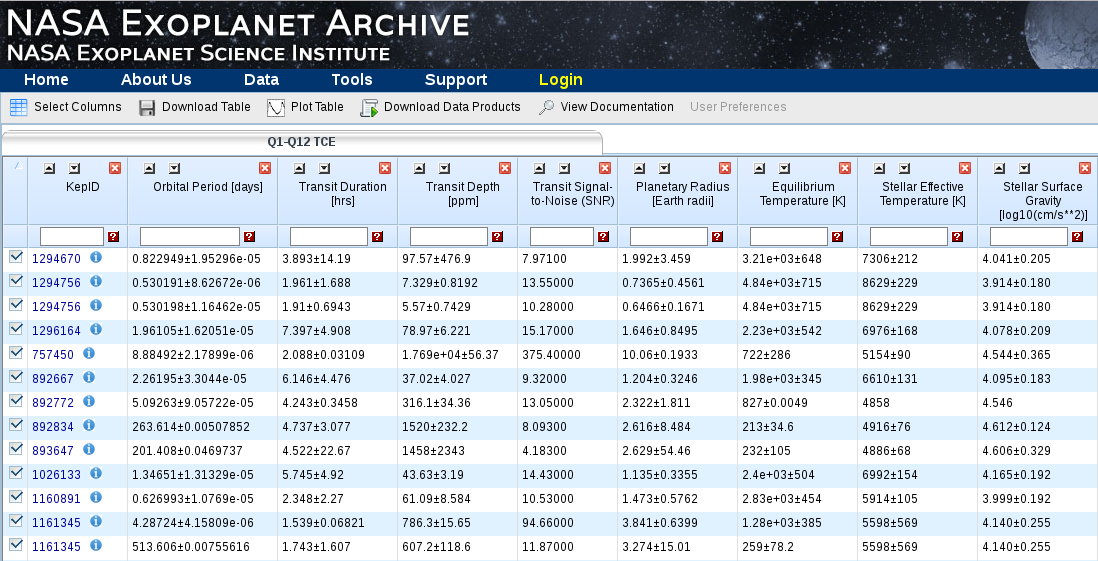
\includegraphics[width=0.8\textheight]{img/TCECatalog.png}
        \caption{Threshold Crossing Event Catalog:  \url{http://exoplanetarchive.ipac.caltech.edu/cgi-bin/TblView/nph-tblView?app=ExoTbls&config=q1_q12_tce}}  \label{fig:tcecatalog}
\end{center}
\end{figure}

Figure \ref{fig:tcecatalog} show a sample of TCE datalog from Exoplanet Archive from  NASA Exoplanet Science Institute. This is an interactive table that has exoplanet archive including information provided by the original sources. Each row that has unique KeplerID is a TCE. In Figure \ref{fig:tcecatalog} show only a few columns out of many. Each column is an observed or a computed data point that related to the given TCE. Using the upper left hand "Select Column" menu, we can select any fields to appear on the table. By hovering over a KeplerID, you can explore more data that is belong to this particular TCE (show in Figure \ref{fig:tcecatalogdetail}). Kepler target overview page show more complete stellar parameters including stellar 2MASS images. Kepler TCE Overview page shows in-depth details of the TCE, this includes Kepler data validation reports and Kepler Planet Detection Metrics and time series data including various downloading options. We can download all the time series data from these catalogs. 

\begin{figure}[!h]
\begin{center}
        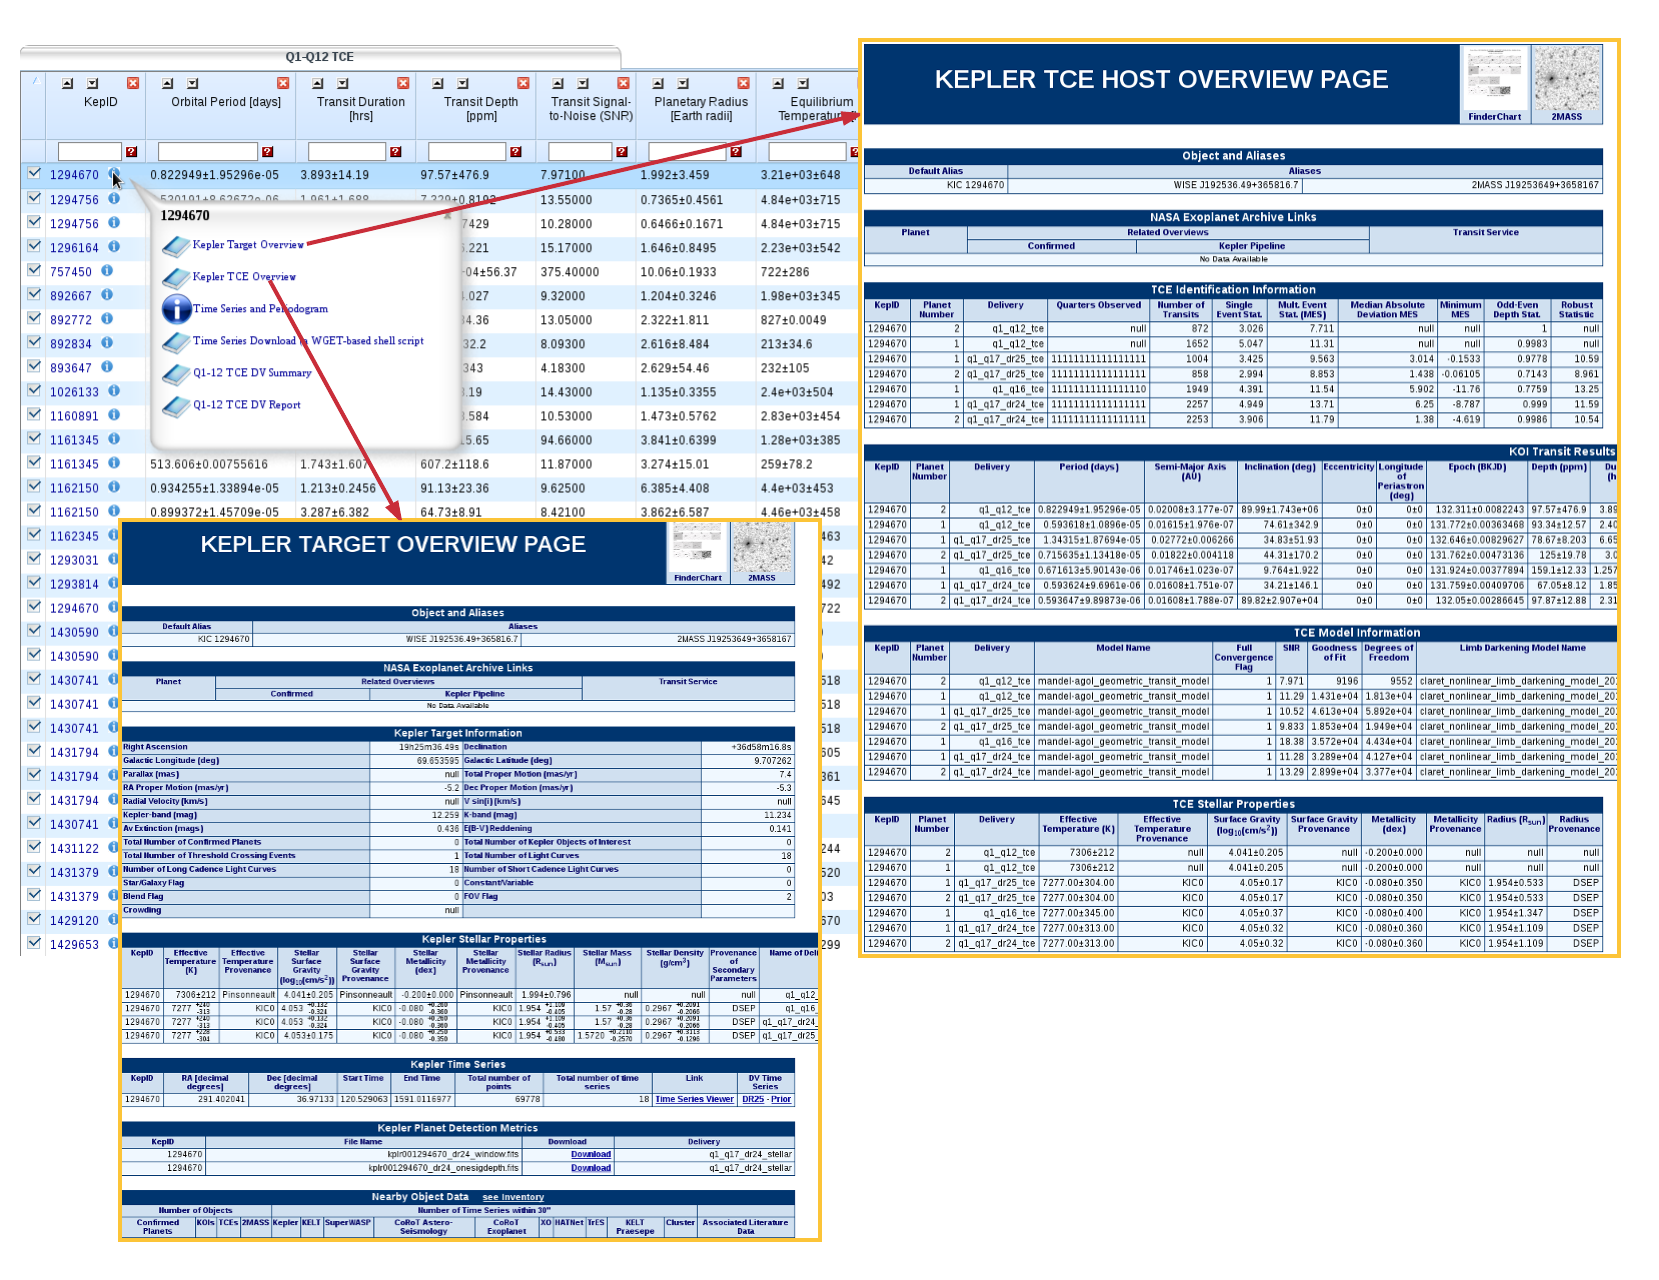
\includegraphics[width=0.8\textheight]{img/tceoptions.png}
        \caption{Threshold Crossing Event Catalog Details}  \label{fig:tcecatalogdetail}
\end{center}
\end{figure}

\section{TCE Attributes}
\label{label:tce_attributes}

Initial TCE attribute set contains 237 attributes that are based on the wavelet matched filter use by TPS, transit model fitting, difference image centroids, and some additional tests. Each of these attributes has different strength of prediction values. The importance of these attributes is selected using historical literature on attributes and performing a Principal Component Analysis. We discuss some of the most important attributes in this section.

\section{Transit Fit Parameters}

This paper presents exact analytic formulate for the eclipse of a star described by quadratic or nonlinear limb darkening. The Kepler Project derives transit parameters from best-fit parameters produced by this analytic formula. Some of the transit parameters are calculated directly; others are derived from the best-fit parameters. Limb-darkening coefficients are fixed and pre-calculated from host stellar properties.  


\subsection{\emph{tce\_ror}: Ratio between planet radius and stellar radios}
\emph{tce\_ror} attribute calculated by planet radius divided by its hosting the stellar radius. Both planet and stellar radius are in Eath-radii units. Plot \ref{plot:planet_star_radius_ratio} show the histogram of the \emph{tce\_ror} attribute in the TCE catalog (x-axis is in log scale and y-axis is in linear)


\begin{figure}[!h]
\begin{center}
        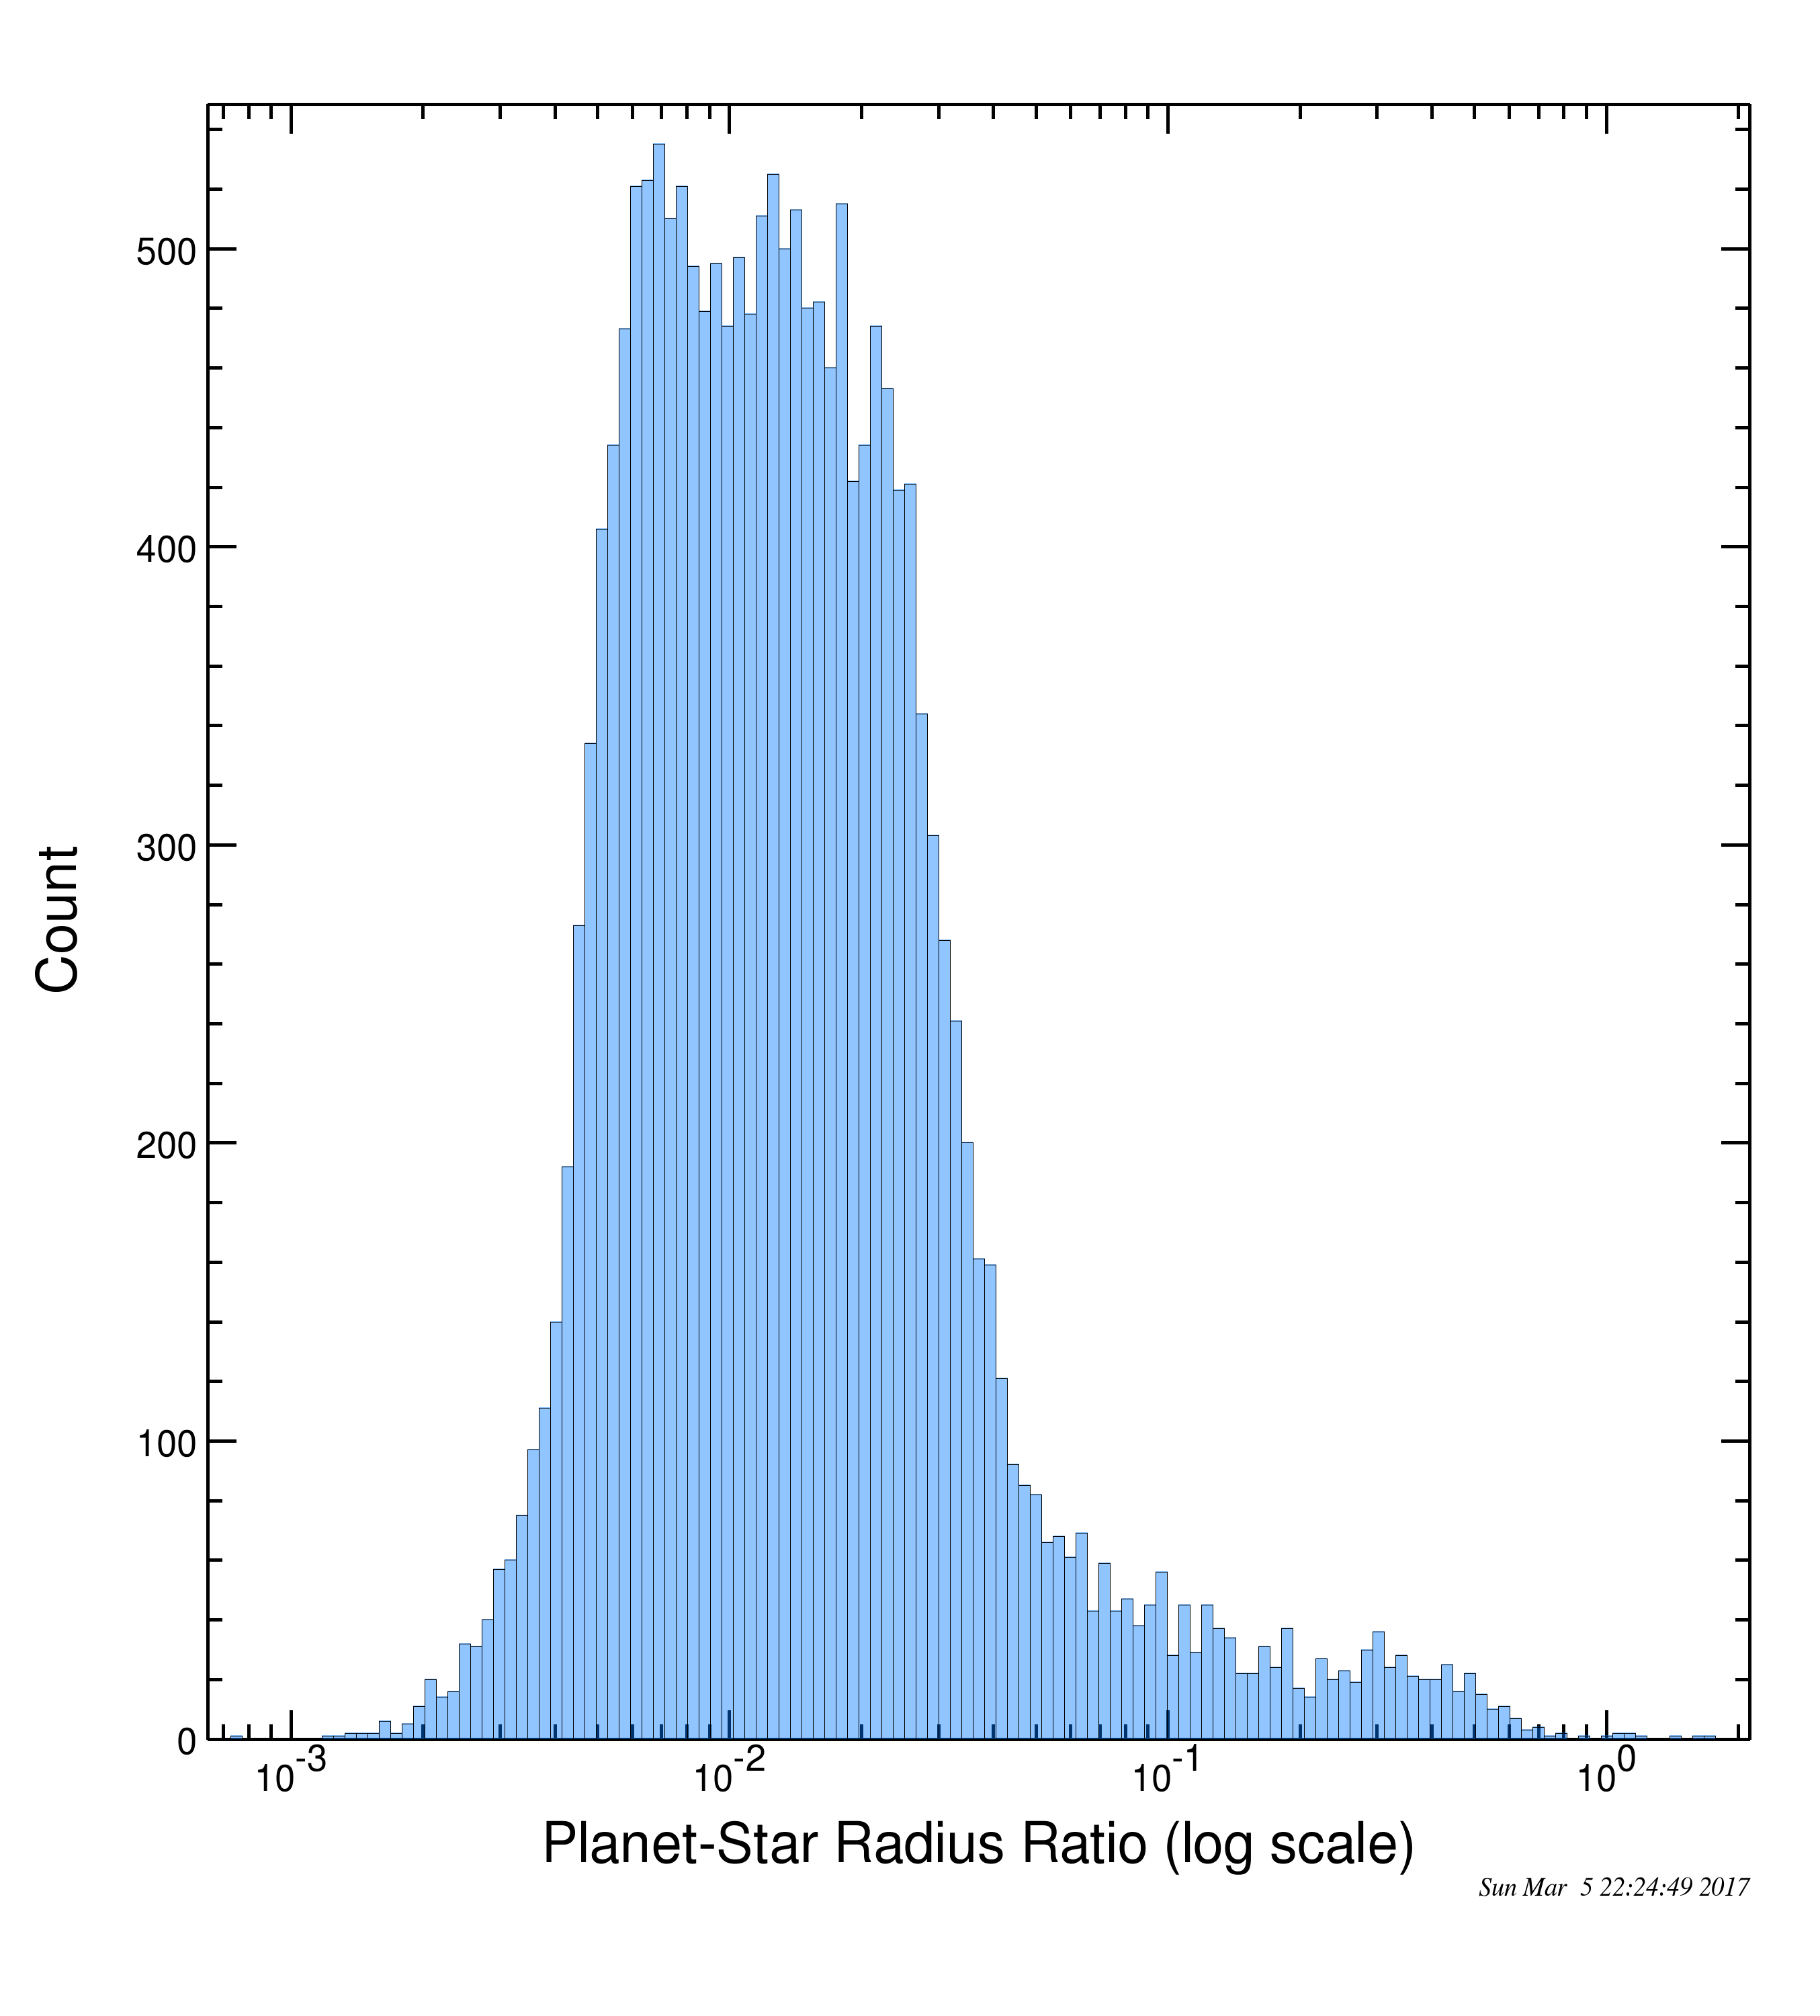
\includegraphics[width=0.5\textheight]{img/planet_star_radius_ratio.png}
        \caption{Ratio between planet radius and stellar radios}  \label{plot:planet_star_radius_ratio}
\end{center}
\end{figure}

\subsection{\emph{tce\_duration}:  Transit Duration}
tce\_duration: The duration of the observed transits. Duration is measured from the first contact between the planet and star until the last contact. The duration is measured by hours. The plot \ref{plot:transitduration} show the distribution of the transit duration of the TCE catalog. We can observe the most of the transit are fall under 10-hour duration.

\begin{figure}[!h]
\begin{center}
        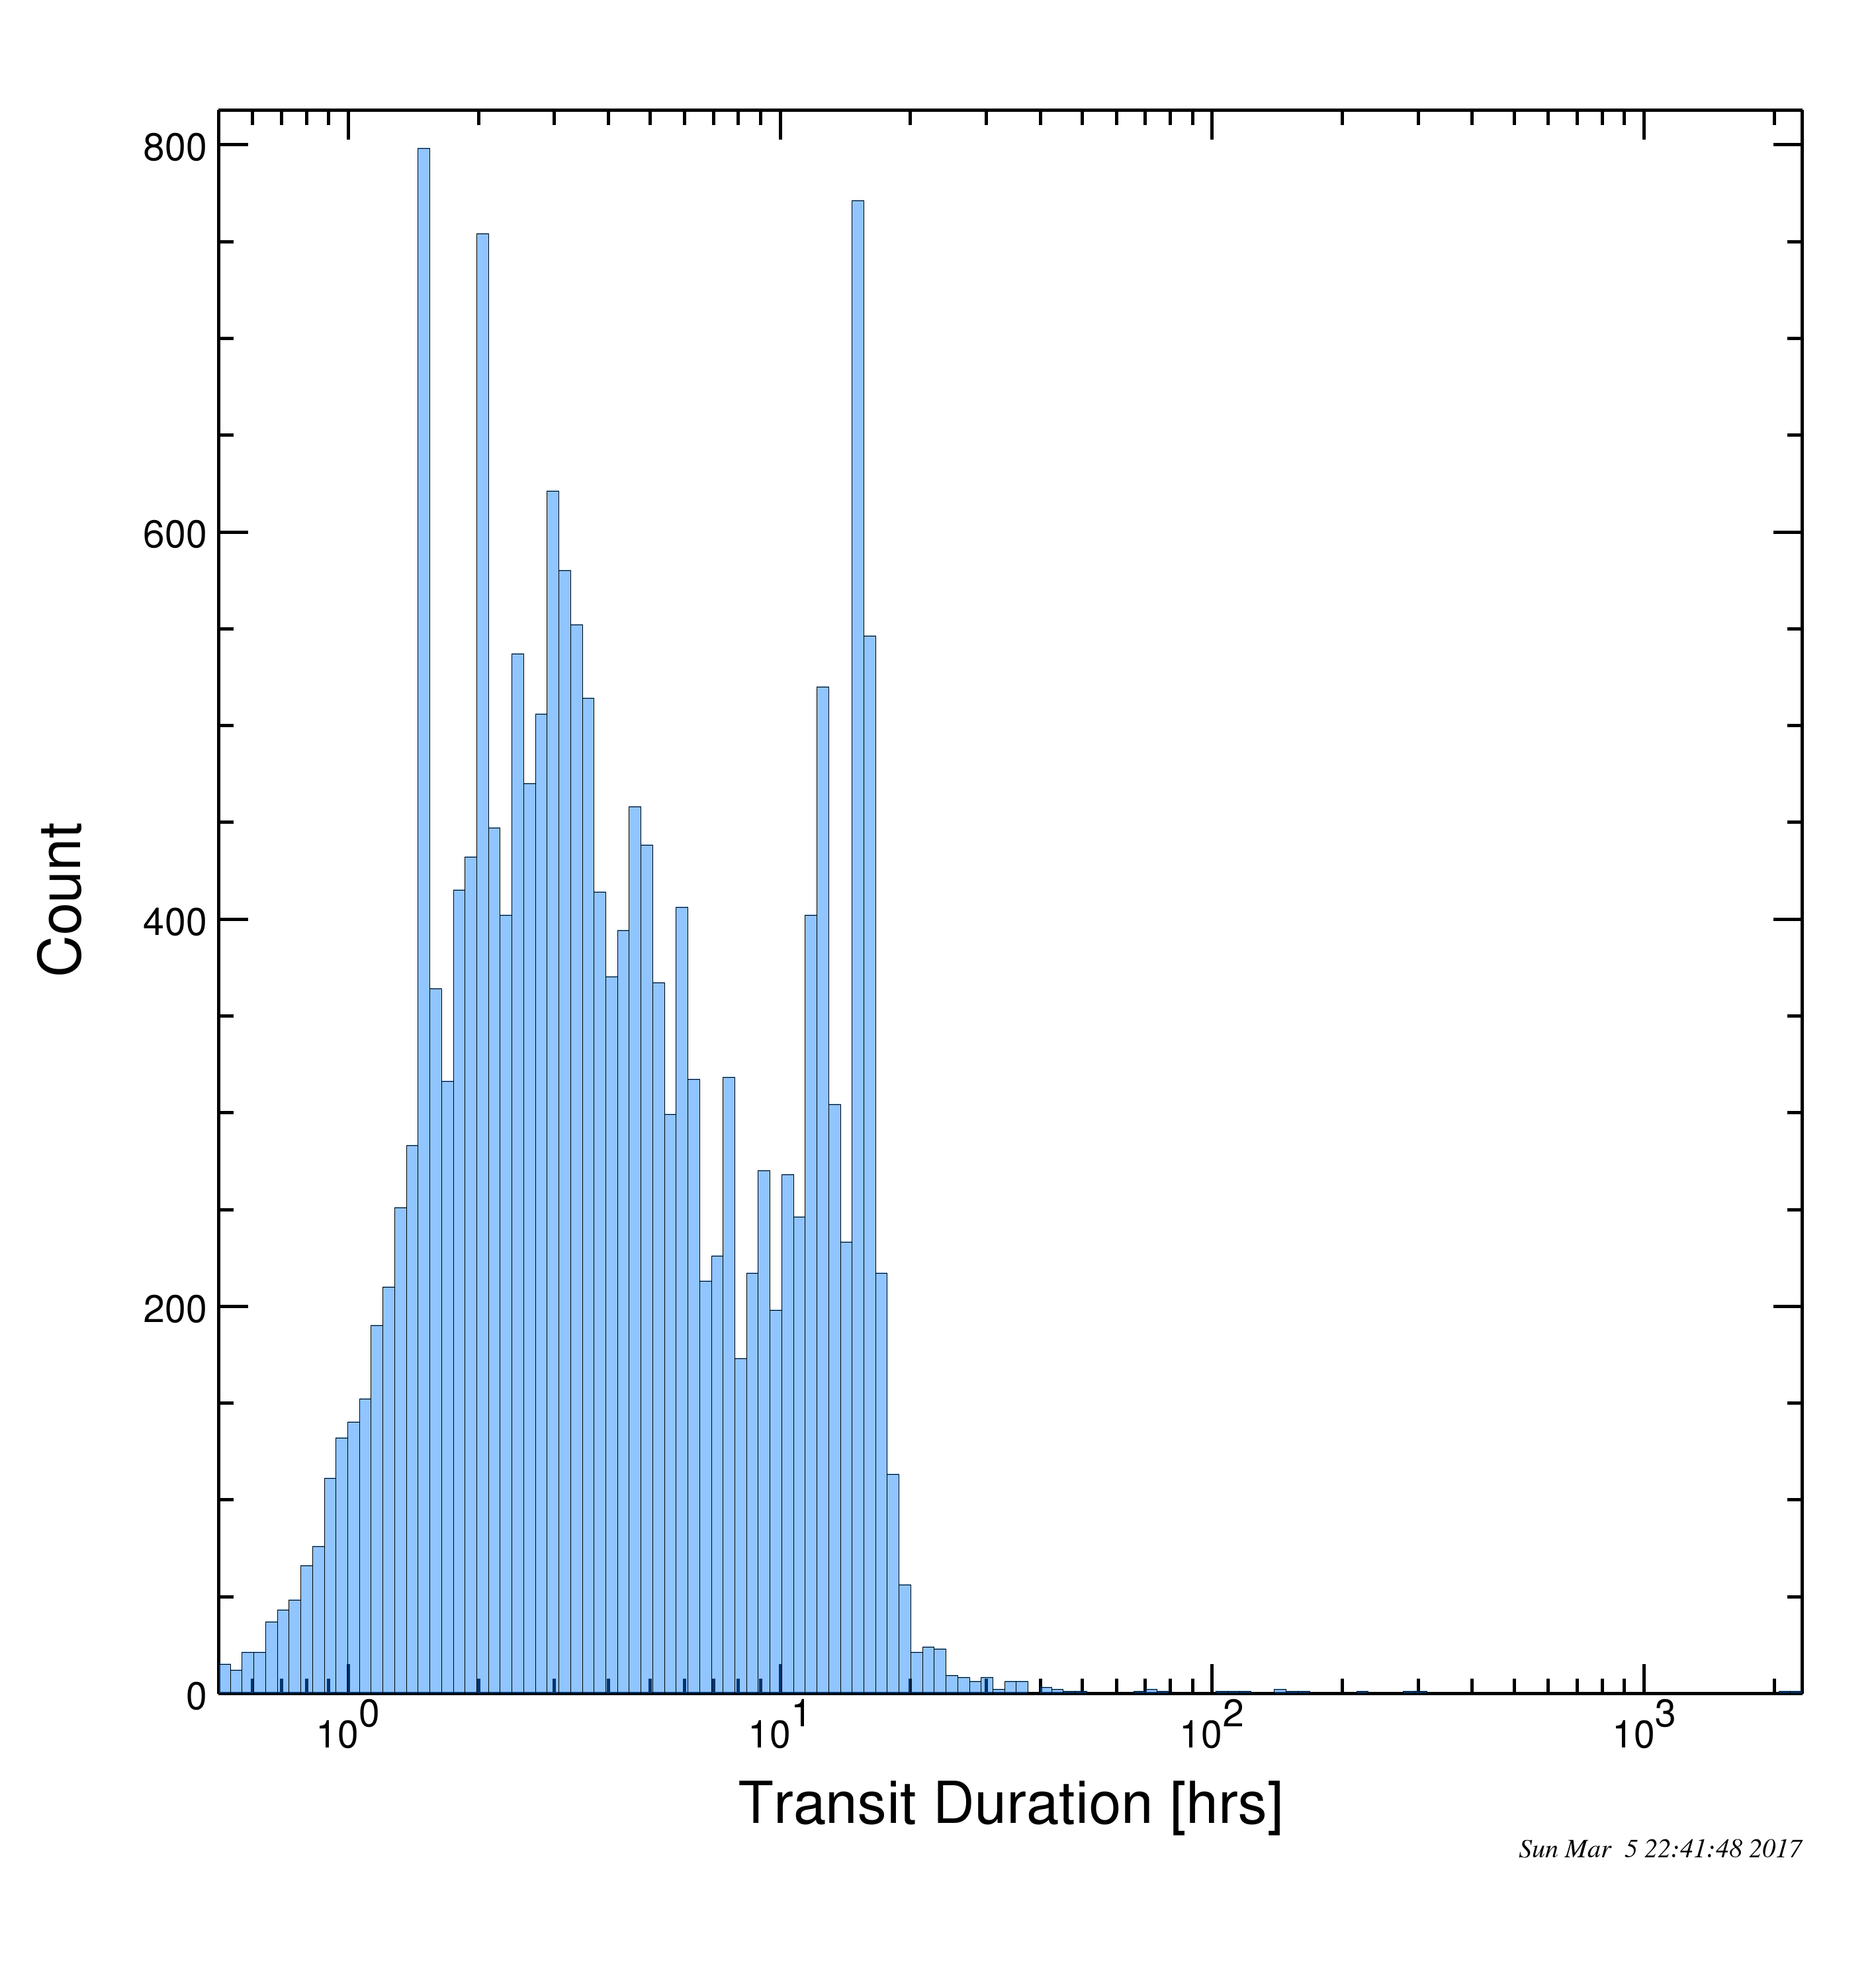
\includegraphics[width=0.5\textheight]{img/transitduration.png}
        \caption{Transit Duration}  \label{plot:transitduration}
\end{center}
\end{figure}

\subsection{\emph{tce\_impact}: Impact Parameter}
tce\_impact: The sky-projected distance between the center of the stellar disc and the center of the planet disc at conjunction, normalized by the stellar radius.

\subsection{\emph{tce\_model\_snr}: Transit SNR}
Transit depth normalized by the mean uncertainty in the flux during the transits. Plot \ref{plot:transitsnr} show the distribution of the SNR. 

\begin{figure}[!h]
\begin{center}
        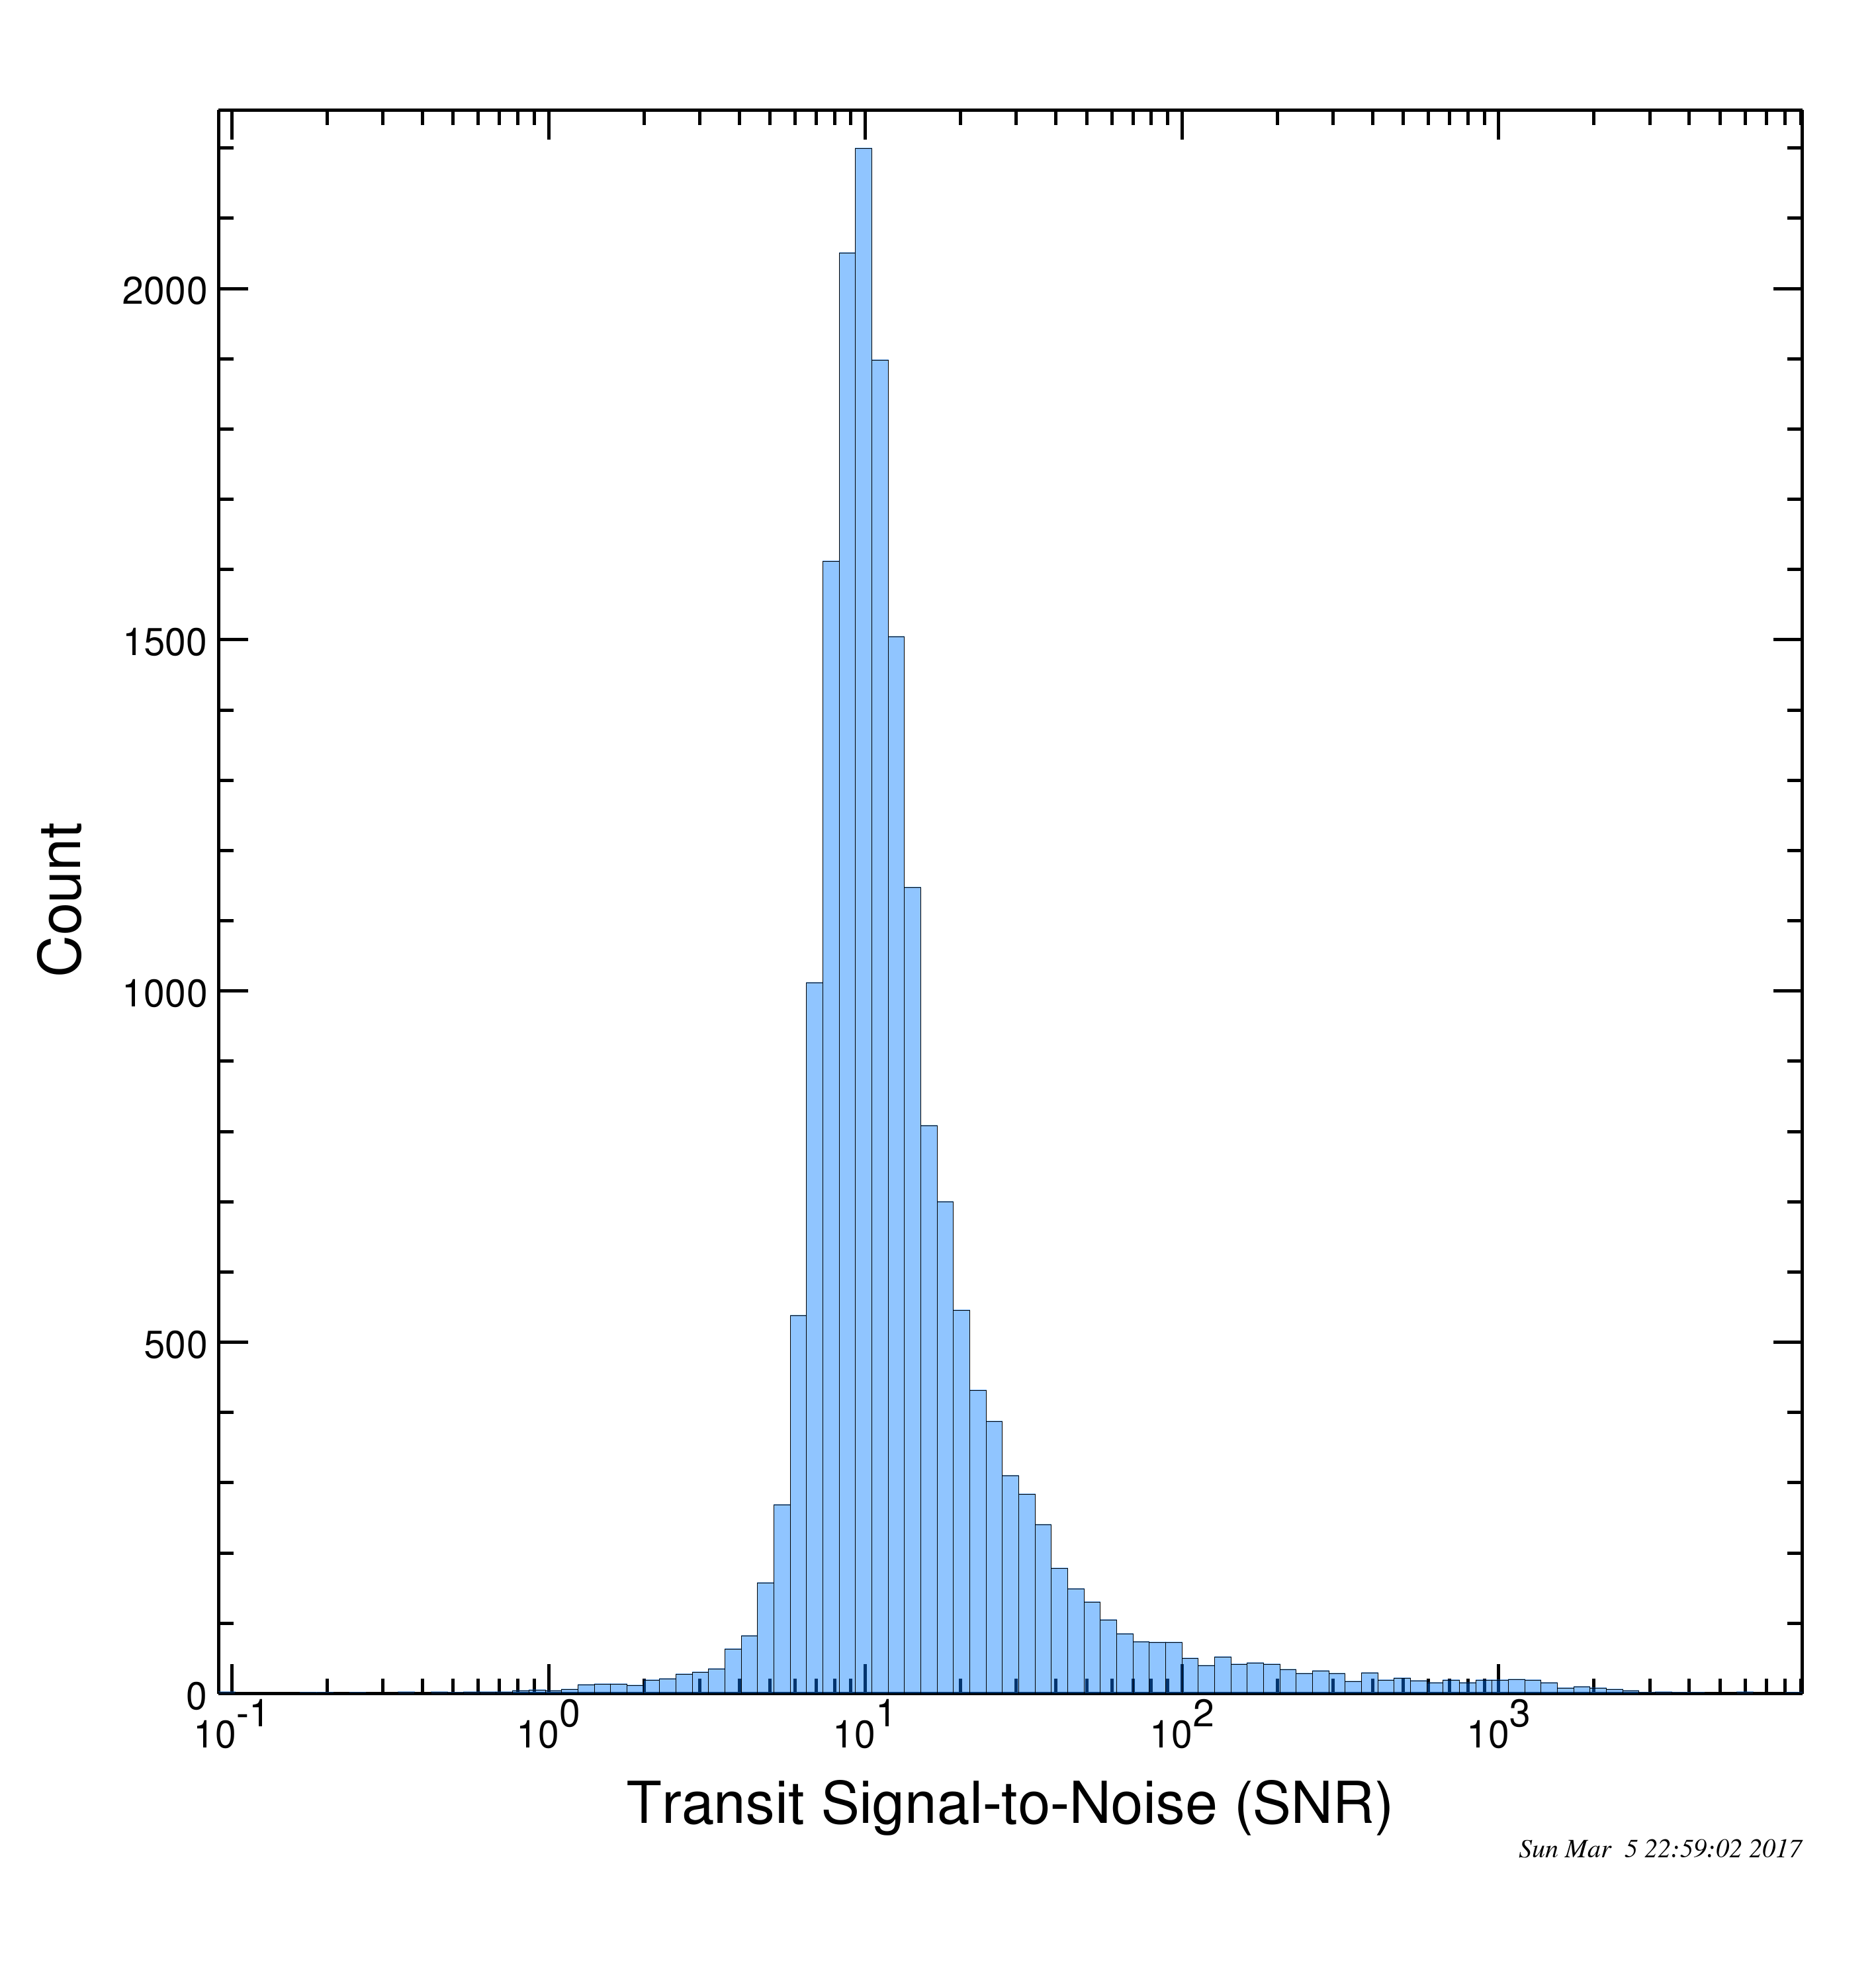
\includegraphics[width=0.5\textheight]{img/transitsnr.png}
        \caption{Transit SNR}  \label{plot:transitsnr}
\end{center}
\end{figure}

\subsection{Stellar Parameters}
Best-fit transit parameters are normalized to the size of the host star. The size of the hosting star is determined by its radius. Physical planet parameters may be derived by scaling to the star's size and temperature. Stellar effective temperature, surface gravity, metallicity, radius, mass, and age should comprise a consistent set. This section describe and visualize some of the stellar parameters from the TCE catalog.

\subsection{\emph{tce\_steff}: Stellar Effective Temperature (K)}
Plot \ref{plot:stellartemp} show the photospheric temperature of the stars in the TCE catalog. Kepler mission target sun-like stars and the photospheric temperature of the sun is 5,775 K. If we plot the sun on the \ref{plot:stellartemp}, it will fall close to the apparently large number count that shows on the plot. This \ref{plot:stellartemp} show the TCE catalog stellar temperatures are falling between 3000K and 17000K 


\begin{figure}[!h]
\begin{center}
        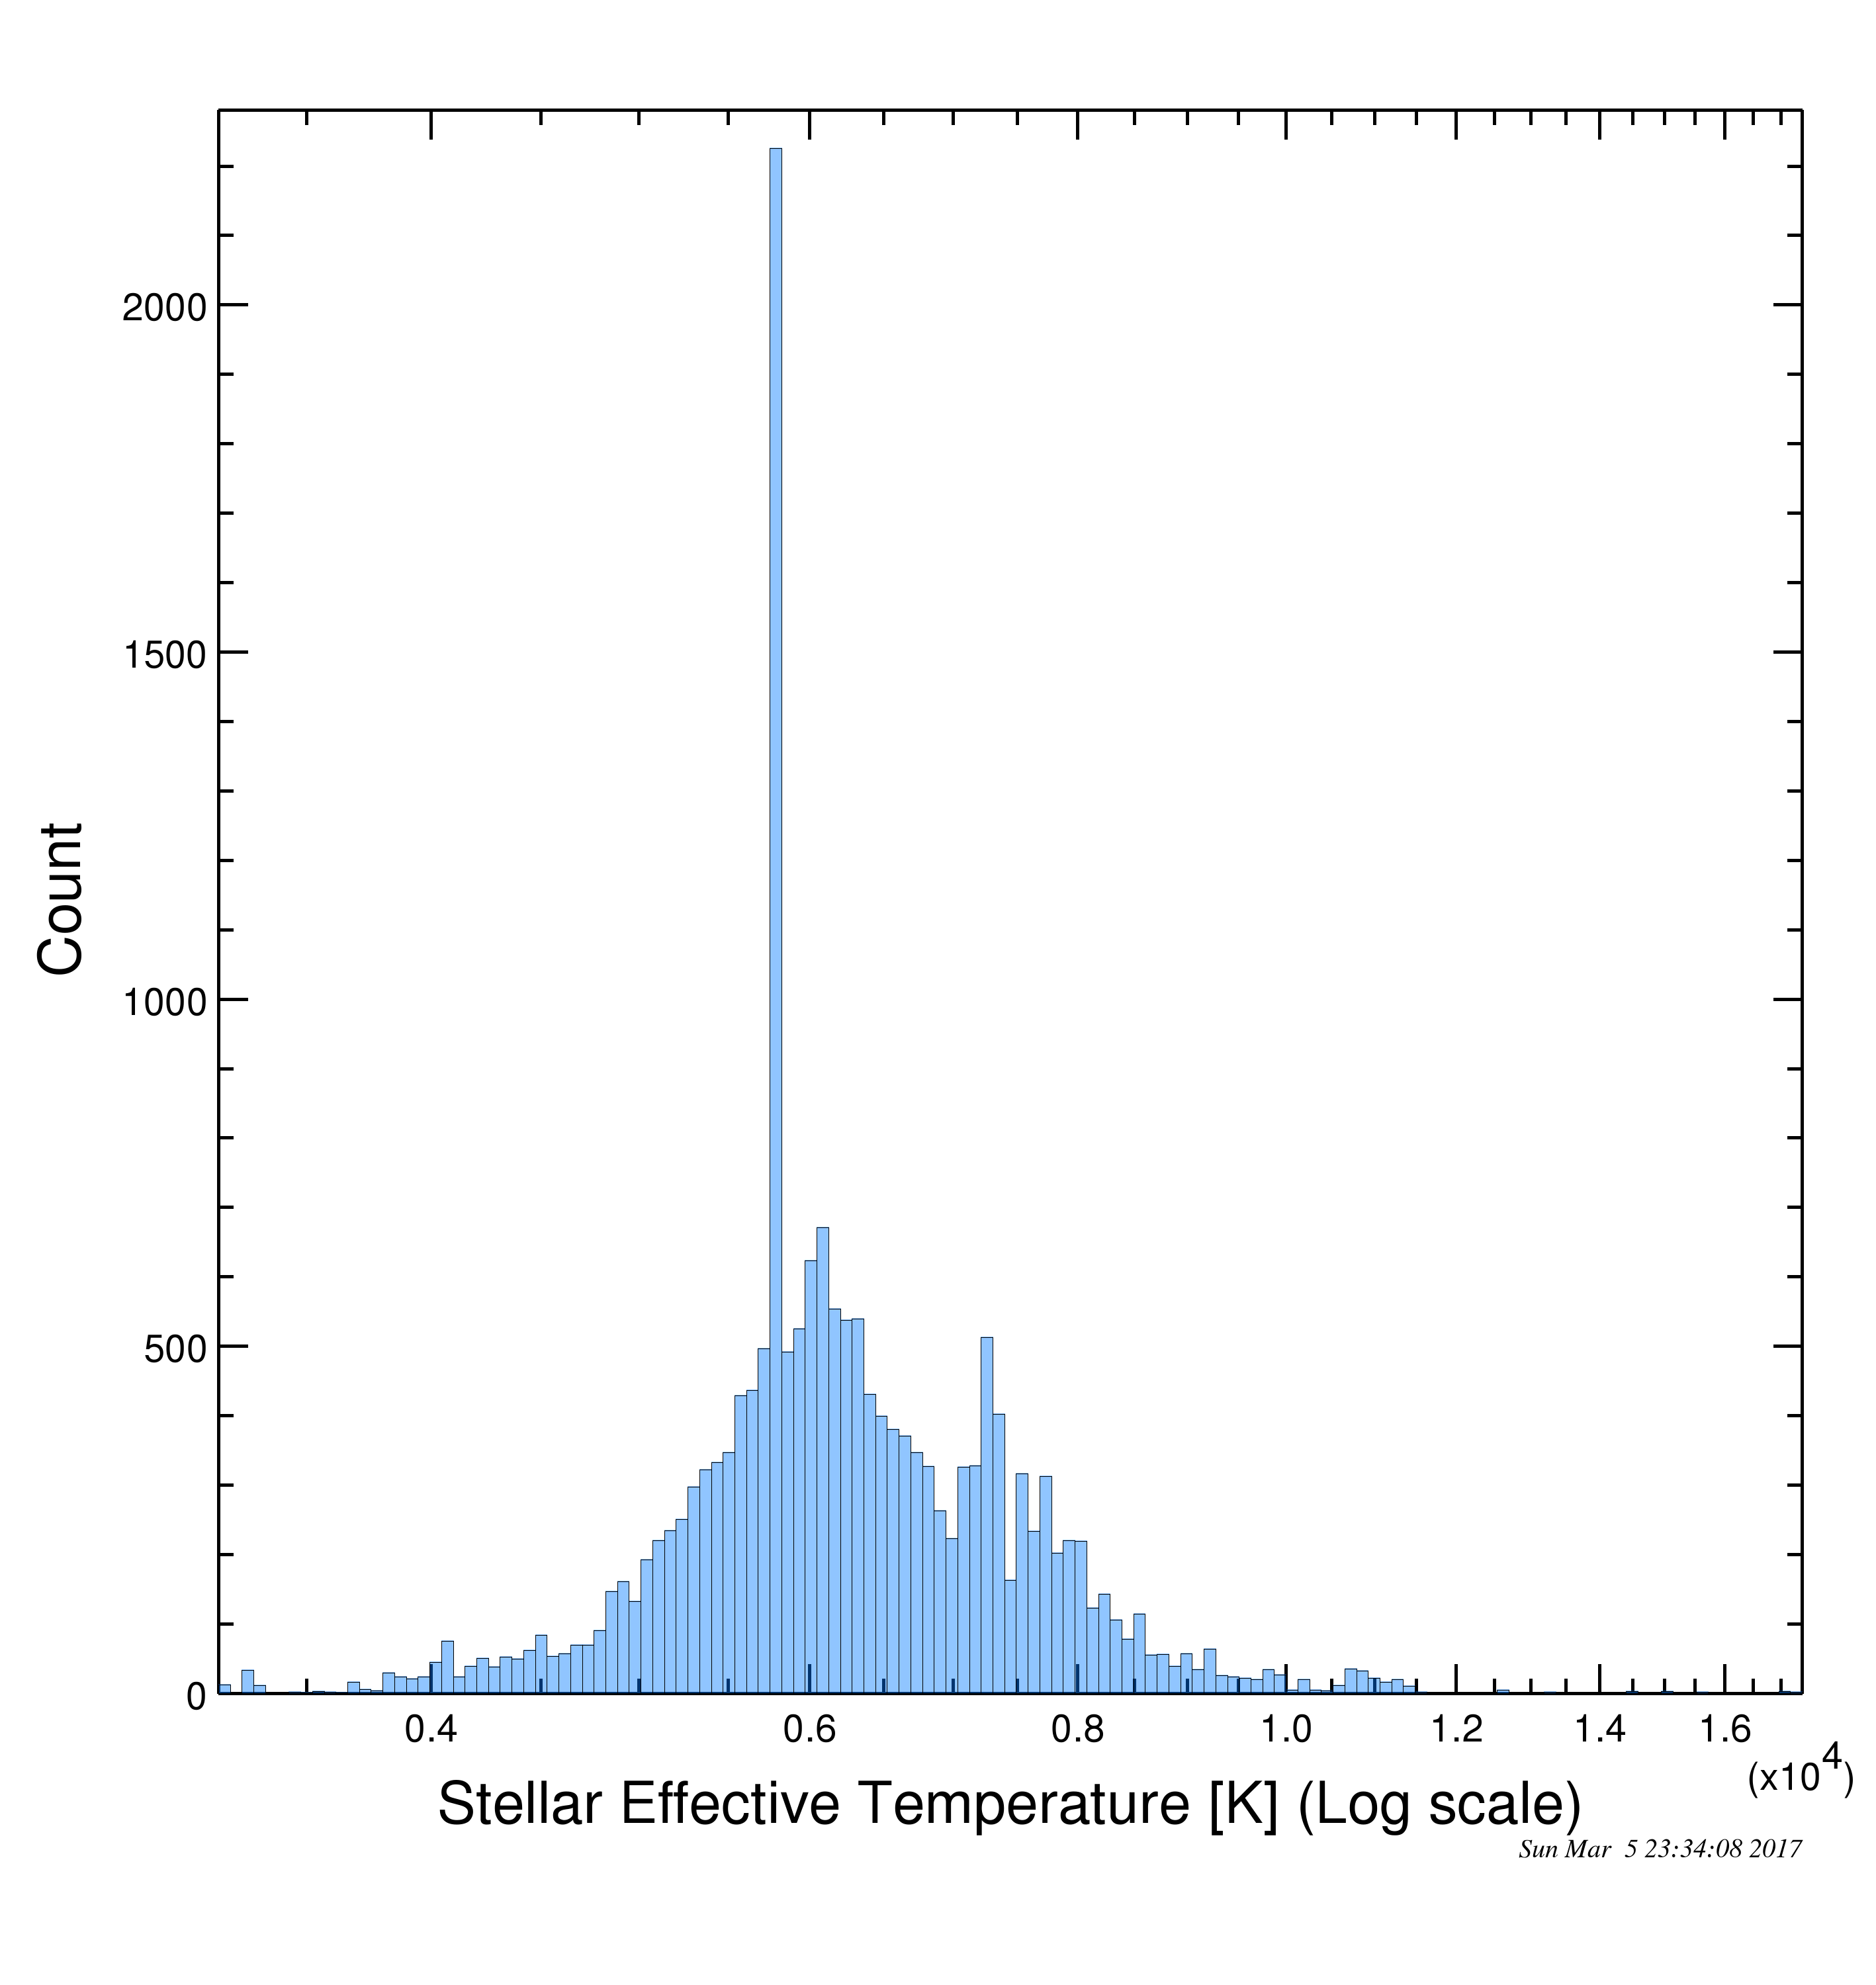
\includegraphics[width=0.5\textheight]{img/stellartemp.png}
        \caption{Stellar Effective Temperature (K)}  \label{plot:stellartemp}
\end{center}
\end{figure}

\subsection{\emph{tce\_slogg}: Stellar Surface Gravity}
The base-10 logarithm of the acceleration due to gravity at the surface of the star. The surface gravity of our sun is 274.0 cm/$s^{2}$ (4.44 log10(cm/$s^{2}$)). Plot \ref{plot:stellargravity} show the distribution of the TCE catalog stellar surface gravity. 

\begin{figure}[!h]
\begin{center}
        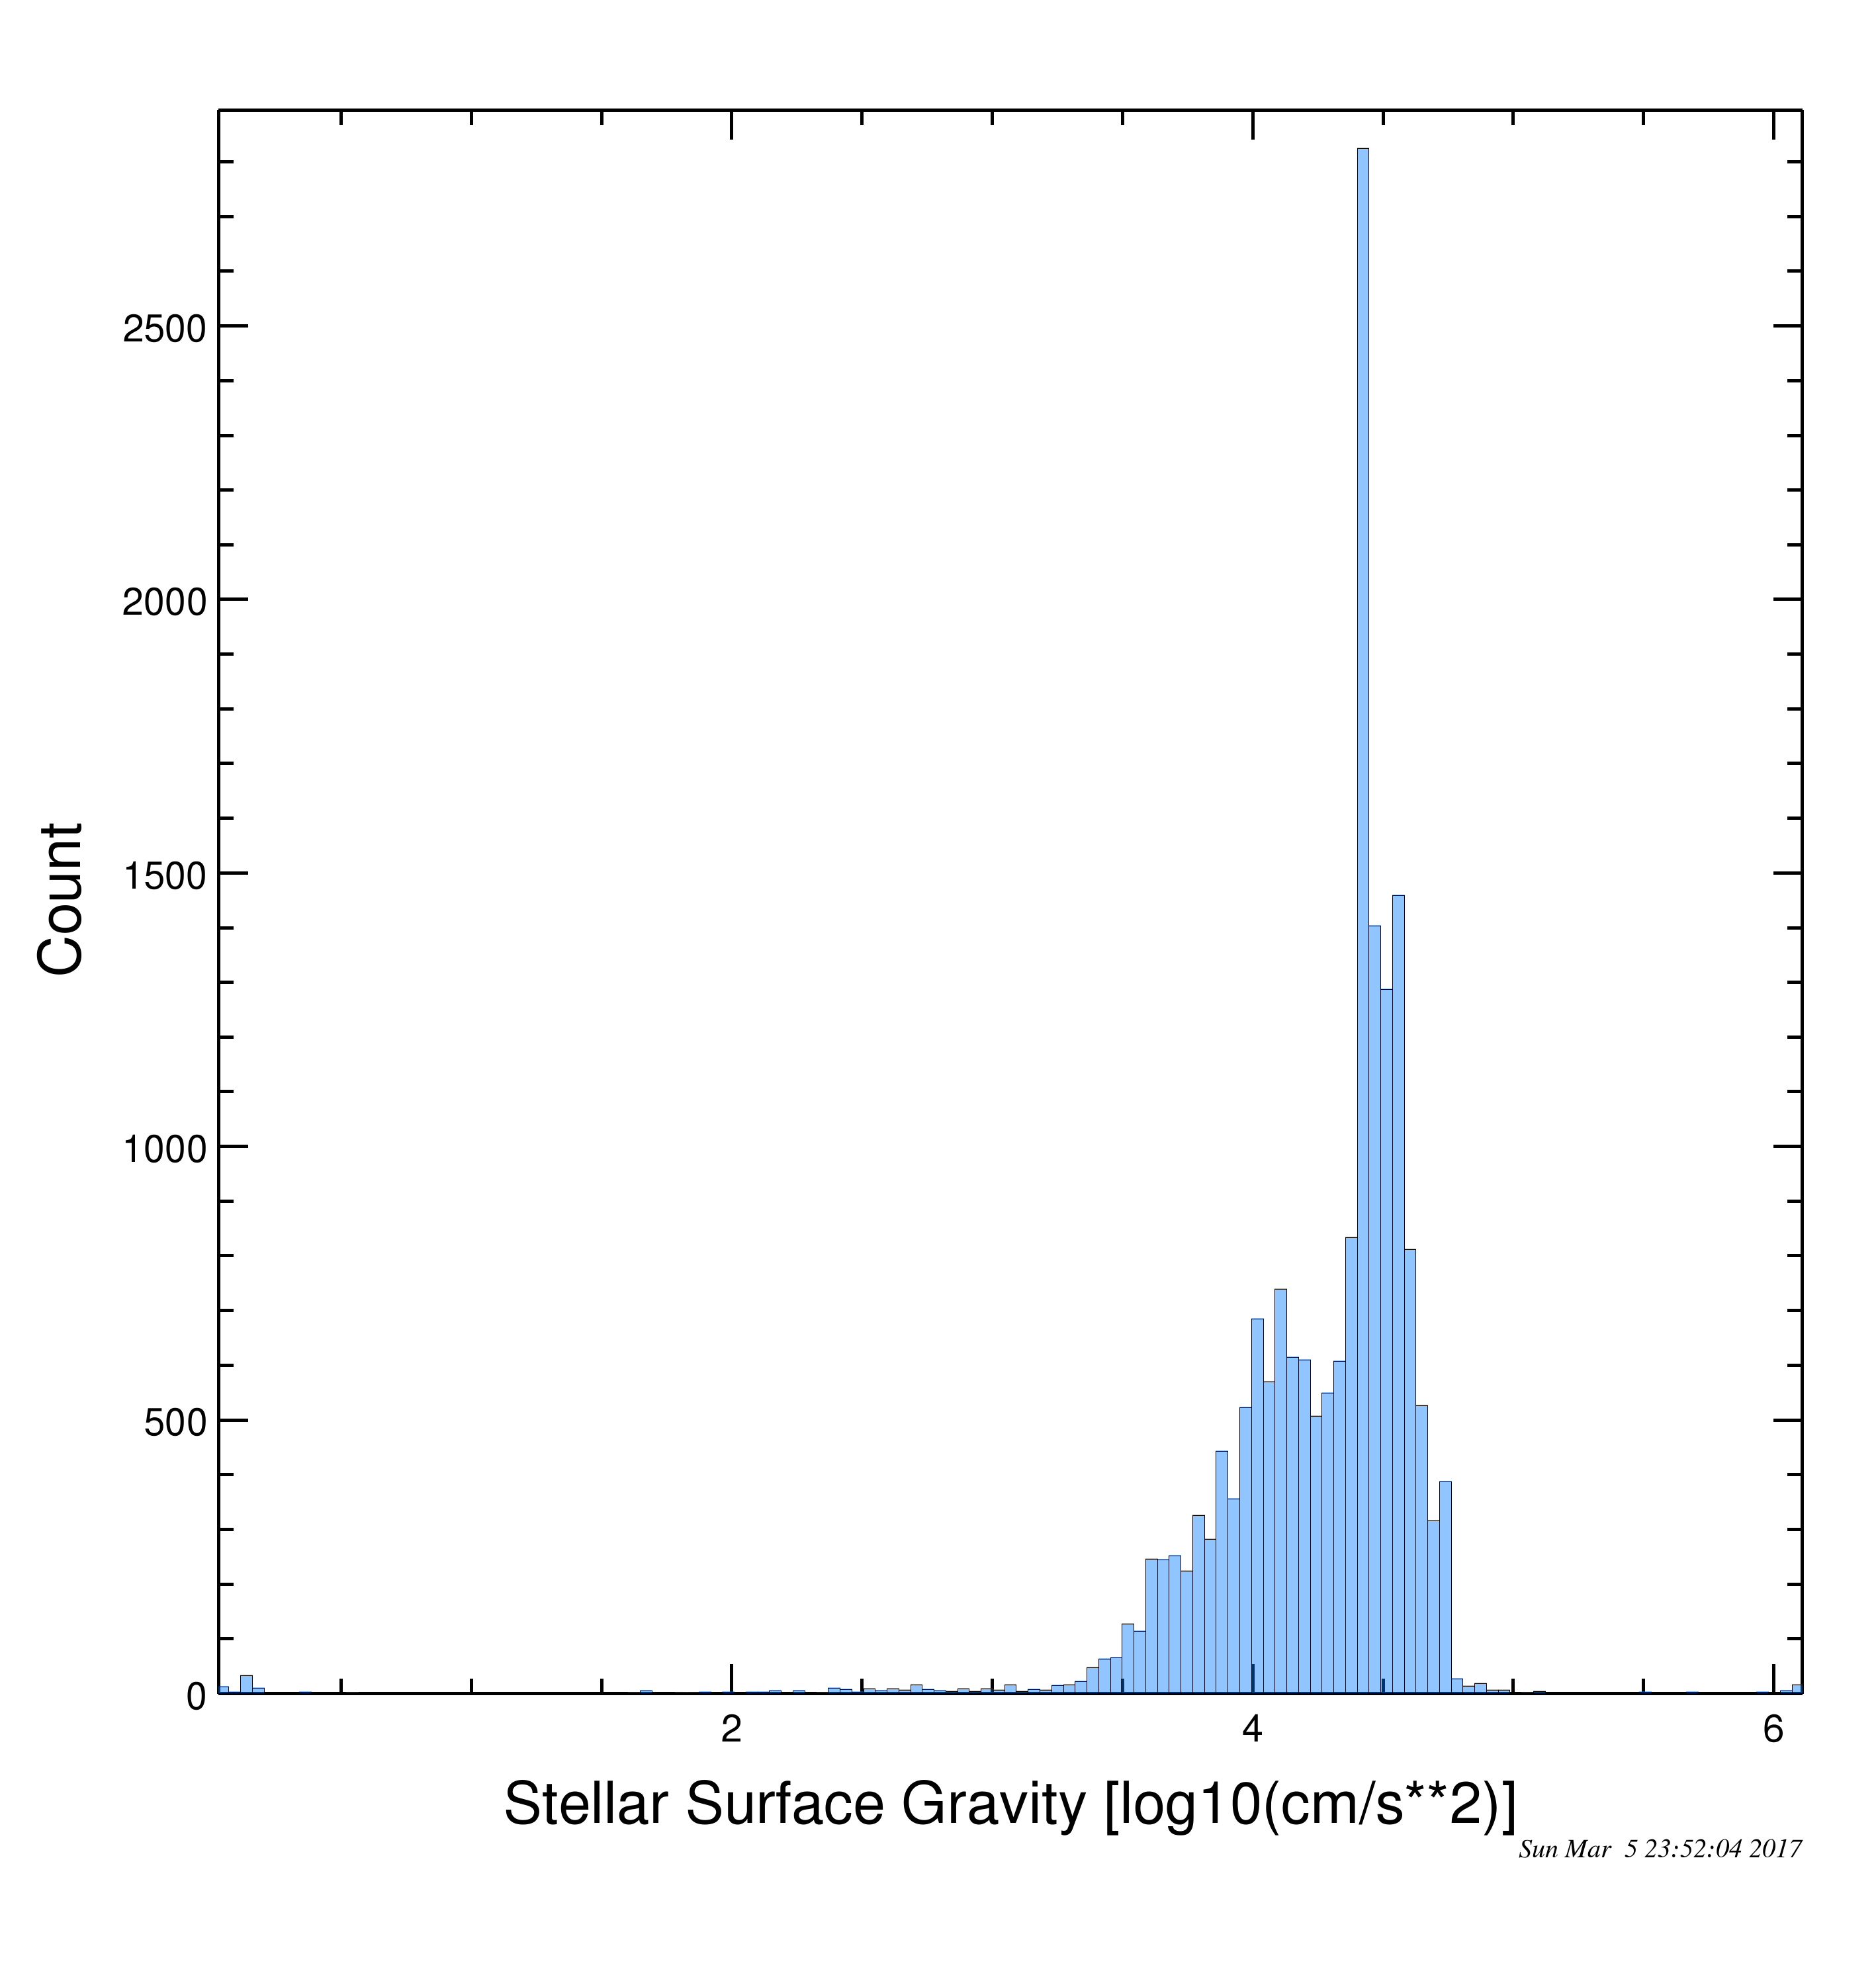
\includegraphics[width=0.5\textheight]{img/stellargravity.png}
        \caption{ Stellar Surface Gravity log10(cm/$s^{2}$)}  \label{plot:stellargravity}
\end{center}
\end{figure}


%\todo{Data Exploration}
%\todo{- Explain TCE Catalog in detail - show some samples, some of this already done}.
%\todo{- Explain the attributes in the dataset - may be use a table with detail description, try to visualize some of the attributes}
%\todo{- Missing data - from the paper, this is already done}
%\todo{- remove the weak attributes}
%\todo{- Explain the classification labels in the dataset - this is already done}
%\todo{Algorithms and Techniques}
%\todo{- Explain PCA indetail }
%\todo{- Explain CNN in detail}
%\todo{Benchmark - define the benchmark and thresholds - this is already done}